\section{Mechanical Layout and Signal Readout of the ME1/1 Chambers}
\label{app:me11}

The ME1/1 is the first muon station of CMS Endcaps~\cite{CMS:1997dma} in very forward region $2.43 < |\eta| < 1.55$. It is composed of $36$ Cathode Strip Chambers (CSC)~\cite{Acosta:2000ty, Ershov:2006sf}, in each Endcap (see Fig.~\ref{fig:CMS_muon_system}). The ME1/1 CSC should provide very good spatial resolution of 75 $\mu$m per station in order to achieve the required momentum resolution in the endcap muon system. This spatial resolution should be delivered in the presence of a strong axial magnetic field in excess of 3 Tesla. The chambers must provide efficient pattern recognition and matching with the inner tracker. The chambers should be very fast in order to identify the bunch-crossing. Their recovery time should be also very fast because the chambers will operate in the presence of the highest particle background rate in the CMS Muon System, up to 1 kHz/cm$^2$, which corresponds to a rate of 100 kHz per cathode readout channel.

The design parameters of the ME1/1 CSC are optimized to meet the specified requirements. The ME1/1 CSC layout is shown in Fig.~\ref{fig:me11_layout} and the basic chamber parameters are presented in Tab.~\ref{tab:me11}. It is a unit of 6 layers of identical proportional chambers of a trapezoidal shape with a cathode strip readout. Each layer is formed by 2 cathode electrodes: strips and continuous plane, having a gap of $7$~mm. The radial strip structure of one ME1/1 CSC covers an angle of $\phi = \pm 5.42^{o}$ to provide an overlap with the neighboring chambers. The anode wires are placed in the middle of the gap. To compensate for the effect of the CSC spatial resolution deterioration due to the presence of the strong axial magnetic field at a nominal value of 3.8 Tesla (Lorentz effect) the anode wires are positioned at an inclination angle of 29$^o$ with respect to and perpendicular to the central strip axis. The groups of 11 anode wires are connected to one readout channel providing radial coordinate measurements, while the interpolation of charges induced on strips gives the precise measurement of $\phi$ coordinate.

The background rate at the bottom of the ME1/1 CSC ($|\eta| \sim 2.4$) is expected to be significantly higher than that at the top ($|\eta| \sim 1.6$). To decrease the counting rate per strip readout channel, the cathode planes of the ME1/1 CSC are mechanically separated into two parts at $|\eta| = 2.09$. The bottom part ME1/1a ($2.09 < |\eta| < 2.43$) has 48 strips and the top part ME1/1b ($1.55 < |\eta| < 2.09$) has 64 strips. 

Electronics and read out configuration of the signals from cathode strips of the ME1/1 CSC were significantly upgraded during Long Shutdown 1 (LS1) of the LHC in 2013-2015. Signals from the cathode strips are amplified and shaped by seven 96-channel Digital Cathode Front End Boards (DCFEB). Each DCFEB reads out a "tower" of 16 strips from all 6 layers. There are 4 DCFEBs attached to the wide part of a chamber (reading out 64 strips per layer in top region) and 3 DCFEBs attached to the narrow part (reading out 48 strips per layer in bottom region). During upgrade new DCFEBs replaced old CFEBs (not digital). Also before upgrade all 48 cathode strips in bottom part of a chamber were triple-ganged to 16 channels in the electronics for both the trigger and the readout, making hit recognition ambiguous. Only one CFEB was used to read out entire bottom part of the ME1/1 CSC. After upgrade the 48 strips in bottom part of the chambers were unganged and connected to three DCFEBs, removing ambiguity in hit recognition.

Signals from the anode wires are amplified and discriminated by the Anode Front End Boards (AFEB). Each AFEB reads out 16 wire groups from 2 layers of the CSC. The discriminator bits are transmitted to the Anode Local Charge Track (ALCT) board where signals are stored as hits. An ALCT board reads out all 18 AFEBs.

\begin{table}[h]
\caption{Parameters of ME1/1 CSC.}
\label{tab:me11}
\begin{center}
\begin{tabular}{|l|l|c|}
\hline
ME1/1 CSC & Inner radius   & 1060 mm ($|\eta|=2.43$) \\
          & Strips cut radius & 1500 mm ($|\eta|=2.09$) \\
          & Outer radius & 2565 mm ($|\eta|=1.55$) \\
          & Strip channels per chamber & 672 \\
          & Anode channels per chamber & 288 \\
          & Layers per chamber & 6 \\ \hline
Layer     & Strip channels per layer & 112 \\
          & $-$ top part & 64  \\
          & $-$ bottom part & 48  \\
          & Anode channels per layer & 48 \\
          & Number of wires: &  \\
          & $-$ total per anode channel ($1$) & 37 \\
          & $-$ total per anode channel ($2-47$) & 11 \\
          & $-$ total per anode channel ($48$) & 44 \\
          & $-$ total per layer & 587 \\
\hline
\end{tabular}
\end{center}
\end{table}

\begin{figure}[t]
  \begin{center}
    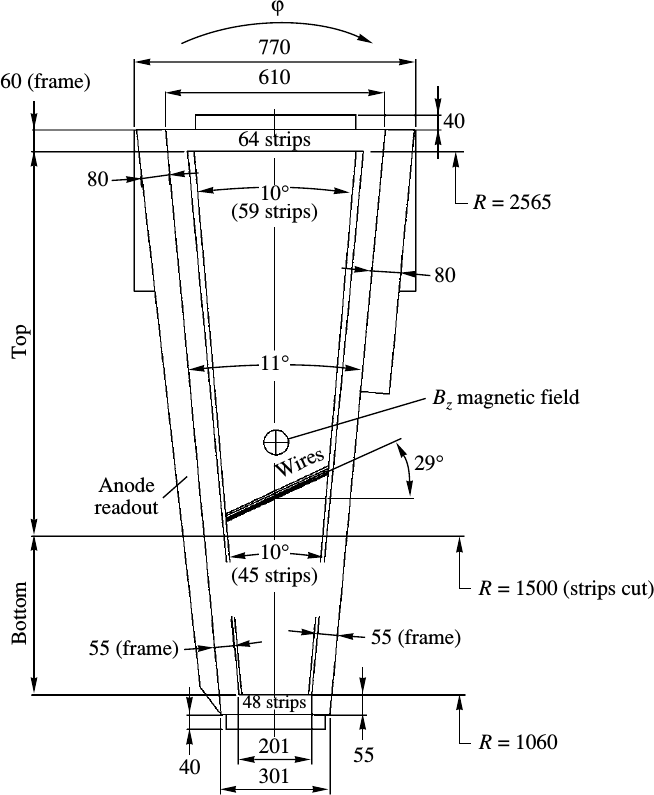
\includegraphics[width=0.52\linewidth]{figures/ME11_layout.png}
    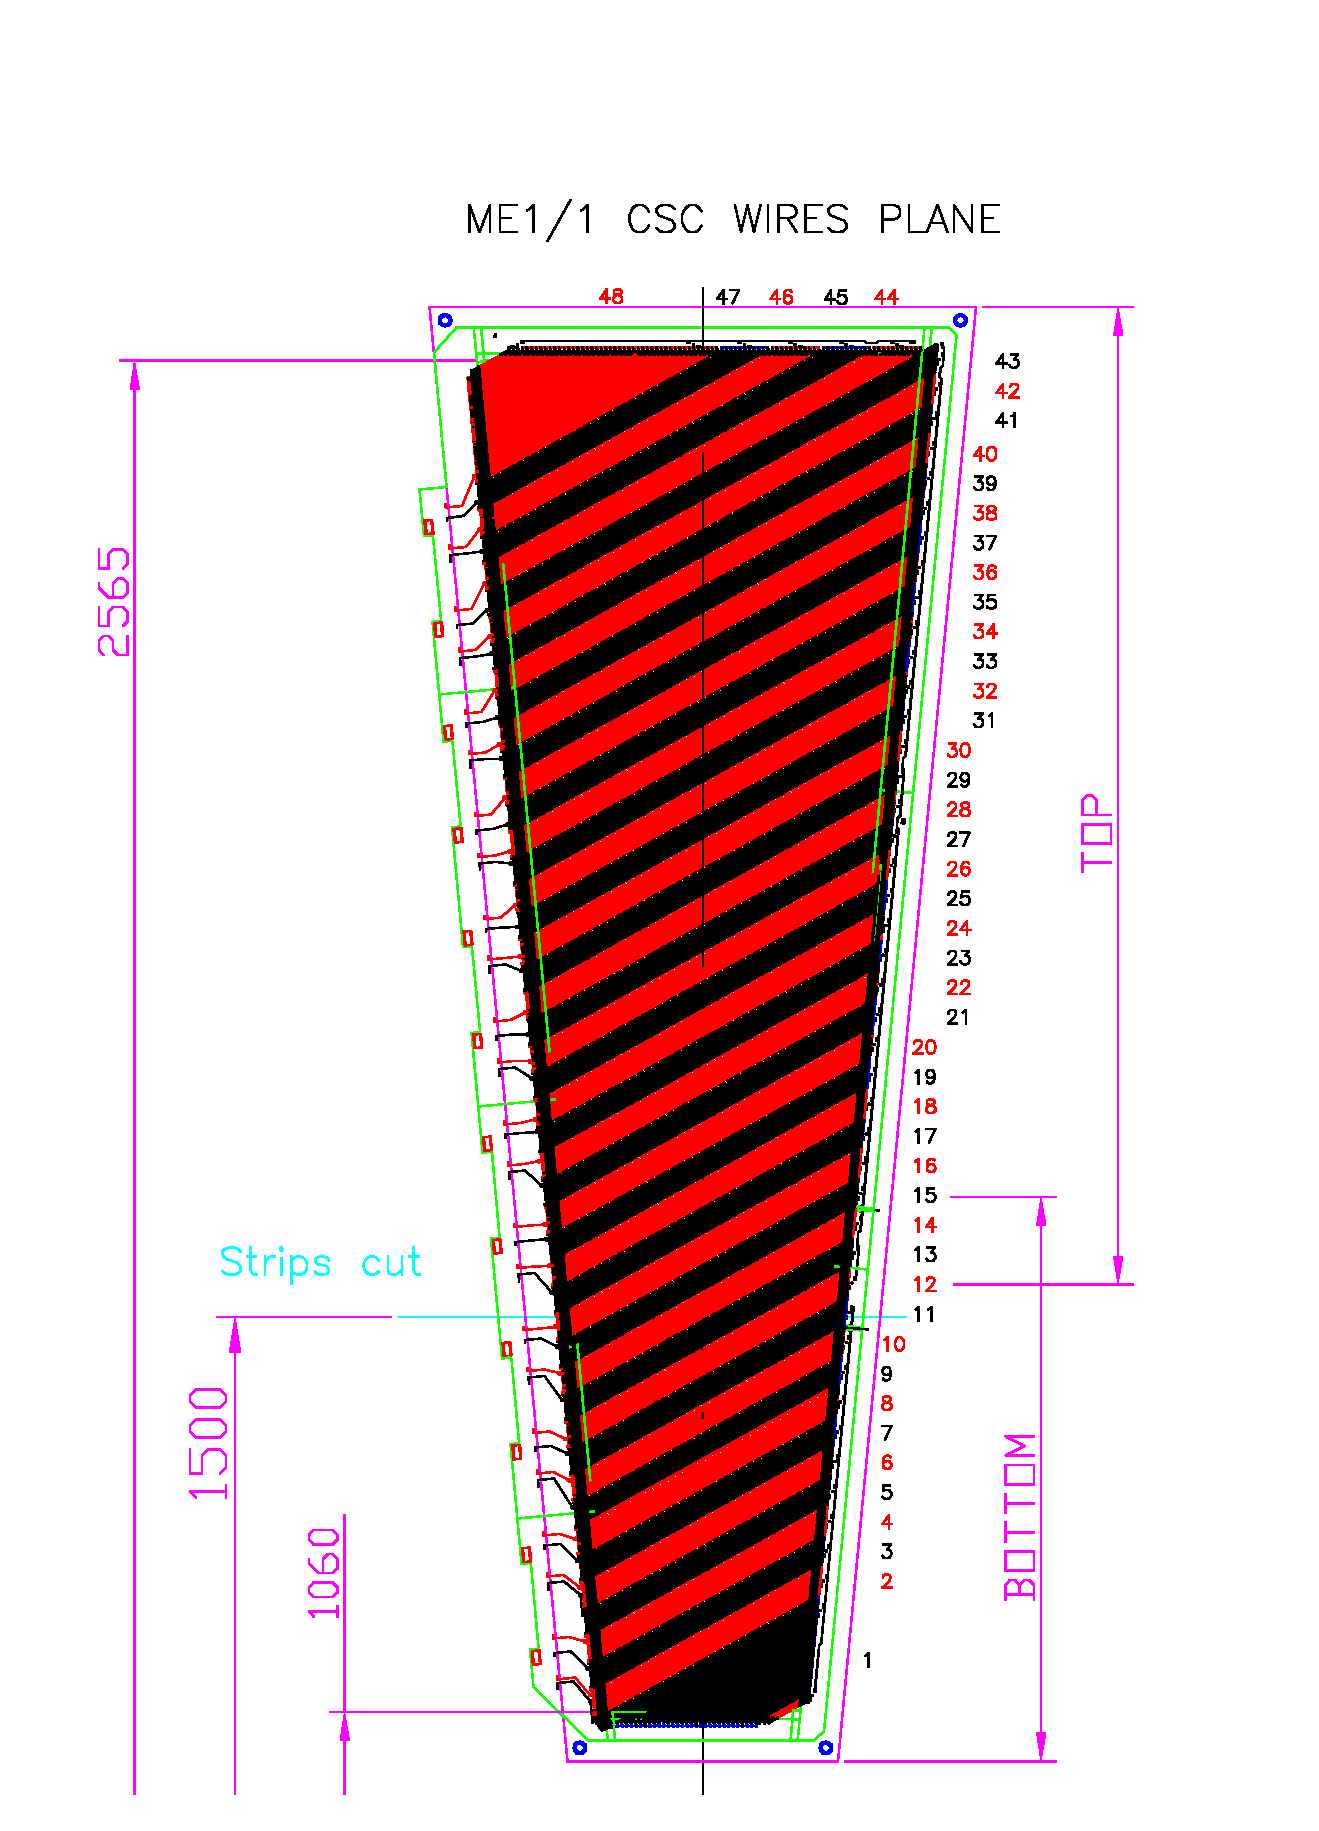
\includegraphics[width=0.47\linewidth]{figures/ME11_wires.pdf}
    \put (-281,3) {\textcolor{red}{$|\eta| = 2.43$}}
    \put (-281,58) {\textcolor{red}{$|\eta| = 2.09$}}
    \put (-281,200) {\textcolor{red}{$|\eta| = 1.55$}}
    \caption{Overall mechanical layout of ME1/1 CSC (left)~\cite{Ershov:2006sf} and layout of 48 anode wire groups positioned at an inclination angle of 29$^o$ (right). All dimensions are in millimeters.}
    \label{fig:me11_layout}
  \end{center}
\end{figure}